\documentclass[12pt]{article}
\usepackage[utf8]{inputenc}
\usepackage{amsmath}
\usepackage{amsfonts}
\usepackage{amssymb}
\usepackage{amsthm}
\usepackage{graphicx}
\usepackage{cite}


\usepackage[colorinlistoftodos]{todonotes}

%\usepackage[mathlines]{lineno}


%\usepackage{endfloat}
%\usepackage[default]{jasa_harvard}    % 	for formatting citations in text
%\usepackage{JASA_manu}

%% CHANGING THE 'AND' IN THE HARVARD BIBLIOGRAPHY PACKAGE TO WHAT IT OUGHT TO BE
%\renewcommand{\harvardand}{and}
%% A FEW NEWCOMMANDS FOR THE CONTENT IN THE EXAMPLE
%% NOT CRUCIAL TO THE USE OF JASA_manu.sty
\newcommand{\Dir}{\mathrm{Dir}}
\newcommand{\ceil}[1]{\lceil #1 \rceil}
\newcommand{\thh}{^\mathrm{th}}
\newcommand{\modtwo}{\mathrm{[mod~2]}}
\newcommand{\thetaof}[2]{\theta \langle #1;#2\rangle}
\newcommand{\Mpa}{M_\mathrm{P,A}}
\newcommand{\Ma}{M_\mathrm{A}}
\newcommand{\rjaccept}{\mathcal{A}}
\newcommand{\RR}{\mathbb{R}}

\theoremstyle{definition}
\newtheorem{defn}{Definition}[section]

\DeclareMathOperator*{\argmin}{arg\,min}
\DeclareMathOperator*{\argmax}{arg\,max}

\begin{document}
\author{Dalla Riva, Giulio V. \and Minh, Tang \and Priebe, Carey E.}
\title{Assessing the importance of species in perturbed food webs through graph embedding}

\maketitle

%\linenumbers
\begin{abstract}
Food-web ecologists have developed and adopted a variety of species importance measures. Here, we introduce and explore a novel measure of this importance, the {\em embedding influence}, which is based on the food-webs Random Dot Product Graph model and is robust to small mispecification in the food-web fine wiring. The embedding influence enable us to predict the overall structural effect of the removal of a species from a food web, e.g., following an extinction event. We show that the distribution of the embedding influence among the species in a food web exhibit an evolutionary signature.
\end{abstract}

\vspace*{.3in}
\noindent\textsc{Keywords}: {Food Webs, Adjacency-Spectral Graph Embedding, Embedding influence, Node Centrality, Network Stability, Trophic Niche Dimensionality.}
\vspace*{.3in}

\section{Introduction}\label{sec:intro}

A food web is the ecological network of who-eats-whom in a community of species: the nodes are species and the arrows between nodes indicate the existence of a trophic relationship, e.g., a predation interaction. A food web can be formalized as a random graph model realization, so that the study of ecosystems can benefit from tools developed in the broad area of complex-network theory.

Biodiversity \cite{wilcox1984situ} has a major relevance for the planet, as recognized by the International Union for Conservation of Nature and the United Nations \cite{hawksworth1995biodiversity}. The increasing human environmental footprint is increasing the extinction risks of single species  and directly affecting the structure of food webs \cite{pimm1984complexity,otto2007allometric,cote2010rethinking,bellard2012impacts,XXX}. The two processes, far from being independent, amplify one the other \cite{saterberg2013high}. This will imply severe economical and social consequences \cite{cardinale2012biodiversity}.

Moreover, budget limitations focus conservation efforts on a selected number of species. It is no surprise, then, that the identification of the species having a crucial role in ecological networks---those species whose extinction or functional loss will most affect the ecosystem---is an important and difficult task for ecologists. This task is made more difficult from the complex and eventually chaotic dynamical behaviour of food webs \cite{MayStability1973,sole2001complexity,XXX}.

In this setting, ecologists have originally developed or adopted from other fields various approach to measure the influence of a species in a food web \cite{estrada2007characterization,martin2010centrality} which span most of the centrality measures based on network structure \cite{harary1959status, freeman1977set,freeman1979centrality,bonacich1987power,brin1998anatomy}. All these measures, however, rely on a rigidly deterministic approach to food webs, albeit the increasing evidence that ecological networks are inherently stocastic \cite{Poisotetal,XXX}. 

In a plea for groups, \cite{allesina2009food} proposed to focus on the functional grouping of species in food web, as recently applied to the Serengeti food web \cite{baskerville2011spatial}.

\paragraph{Random Dot Product Graph}

A natural framework for network partitioning is the stochastic blockmodel graph theory, originally developed for undirected social network analysis  \cite{holland1983stochastic} and subsequently generalised to directed graphs \cite{wang1987stochastic}.  Under this model, each of the $n$ species of a food web are assigned to one of $K$ blocks whose within and between linking probability are given by the model parameters. We do not observe the assignment of the species; rather, we observe the realized adjacency matrix. It has been proved that a consistent block estimator based on the spectral partitioning of the normalized Laplacian of the adjacency matrix exist \cite{rohe2011spectral}, that is the proportion of nodes assigned to the wrong group by the estimator converge in probability to zero as the size of the graph grows to infinity. We will present the definitions in the context of \textit{Random Dot Product} graphs \cite{fishkind2013consistent}, which can be seen as a particular example of stochastic blockmodels.

We will consider the generalization of the latter result to the spectral partitioning of adjacency matrices \cite{sussman2012consistent}. Here we propose a measure, called the {\em embedding influence}, which express the difference between the original food web and the food web derived by the loss, or non-observation, of one of the species. The method doesn't require the knowledge of the number of the blocks but just an upper bound on the rank of the communication probability matrix. The computation of the embedding influence of each node via simple brute force is feasible for food webs of usual size.

In summary, the proposed method consists in computing the estimated parameter matrix for the original observed adjacency matrix, as shown in  \cite{fishkind2013consistent}, removing the species $i$ from the graph embedding and computing the distance of the reduced matrix to the estimated parameter matrix for the modified adjacency matrix obtained by removing from the original food web the species $i$.

 We will apply it to two compilations of the Serengeti food web, namely \cite{baskerville2011spatial} and \cite{de2011serengeti}, the Caribbean marine food web in its original compilation \cite{rezende2009compartments} and to the food web we derived from the latter clustering the species in their families.
 
Finally we will discuss a possible interpretation of the results in terms of species loss, wherein the influence represents how much a food web change its geometry after the lost species extinction, and in terms of non observation of a one species due to possible sampling error during the food web compilation (see \cite[Section 11.2]{rossberg2013food}), wherein the influence represents how much a statistical description of the food web may be different.

\section{Method}
\subsection{Graphs and embedding}\label{secsec:method}

A food web shows the ``resource~$\to$~consumer'' relationship between species in a certain ecosystem. We will also use, in a similar fashion, the  ``prey~$\to$~predator'' jargon. Formally, a food web is a directed graph $G=(V,E)$ which vertices $V$ are the species of the ecosystem and the links $e \in E$ are ordered couples between two species $v_i, v_j$, such that a link $e = (v_i,v_j)$ exists if and only if $v_i$ is a resource of $v_j$, that is $v_j$ feeds on $v_i$ (or, in other words $v_i$ is a prey of $v_j$ and $v_j$ preys upon $v_i$). In general food webs may exhibit loops, i.e. species that prey upon themselves; symmetrical linkings where both $(v_i,v_j)$ and $(v_j,v_i)$ are observed in $E$, i.e. two species mutually preying one on the other; and closed path, although these are rare cases and are omitted for simulation purposes. More generally, the abundance of {\em motifs} (small sized subgraphs \cite{stouffer2005quantitative}) in empirical observed graphs is consistently different from the one which could be expected by most of the random graph null models \cite{stouffer2007evidence}.

The adjacency matrix of a graph $G$ is the matrix $A_G \in \{0,1\}^{n \times n}$ where the $i\mbox{th}$-$j\mbox{th}$ element $A_G^{(i,j)}$ is $1$ if $v_i$ preys upon $v_j$ and is $0$ otherwise.

\subsection{Random dot product graphs}\label{subsec:asge}

Consider a food web $G=(V,E)$, defined as above, with $n$ species, that is $|V(G)| = n$.

In the random dot product model to each species is assigned a {\em latent vector} of dimension $d$ and the probability that an edge $v_i \to v_j$ is given by the dot product of the latent vectors of $v_i$ and $v_j$

Let $R = \left[ R_1, R_2, \dots , R_n \right]^T $ and $L =  \left[ L_1, L_2, \dots , L_n \right]^T$ be $n \times d$ random matrices, where $R_i,L_i \in \RR^d$ for all $i$ are respectively the latent vector of species $v_i$ as a predator and as a prey (we could say that the predation relationship are driven by $d$ traits). The latent vectors $R_i,L_i$ are such that $\mathbb{P}\left( \langle L_i, R_j \rangle \in [0,1] \right) = 1$ for all $i,j$.\todo{There may be another couple of relevant papers published in Ecology: still searching them.}

Conditioned on $L$ and $R$ the entry of the random adjacency matrix $A_G$ are independent and $A_{Gi,j}$ is a Bernoulli random variable of parameter $\langle L_i, R_j \rangle$. Hence, rembembering that $A_{Gi,j}$ takes value in $\{ 0,1 \}$, we have that the probability of observing a certain graph $G$ (which adjacency matrix is $A_{Gi,j}$) is:
$$\mathbb{P}\left(A_G | L, R \right) = \mathbb{P}\left(A_{Gi,j} | L_{i,j}, R_{i,j} \right)$$
$$\mathbb{P}\left(A_G | L, R \right) = \prod_{i \neq j} \langle L_i, R_j \rangle^{A_{Gi,j}}(1-\langle L_i, R_j \rangle)^{1-A_{Gi,j}}$$

A rank~$d$ embedding of a matrix $M \in \RR^{n \times n}$ is the given of a pair of $\RR^{n \times d}$ matrices $\hat{L}_A$ and $\hat{R}_A$ such that the couple $(\hat{L}_A,\hat{R}_A)$ minimizes the Frobenius norm of the difference $M - LR^T$ between all the matrices $L$ and $R$ in $\RR^{n \times d}$.

In particular, when a food web is a realization of a random dot product model and $A_G$ is its observed adjacency matrix, $\hat{L}_{A_G}$ and $\hat{R}_{A_G}$ are an estimate of the latent vectors of the species in the random graph.

Consider a singular value decomposition of $A_G$, that is $A_G = LSR^T$. Hence $L$ and $R$ are real, orthogonal $n \times n$ matrices and $S$ is a $n \times n$ diagonal matrix which non increasingly ordered entries $\Sigma_1, \Sigma_2, \dots , \Sigma_n$ are the singular values of $A_G$. Let $R'$ be the $n \times d$ matrix given by the first $d$ columns of $R$, $L'$ be the $n \times d$ matrix given by the first $d$ columns of $L$ and $\sqrt{S'}$ be the diagonal matrix defined by the square root of the $d$ greatest singular values of $A_G$. Define $\hat{L}$ as $L' \sqrt{S'}$ and $\hat{R}$ as $R' \sqrt{S'}$. Hence the pair of matrices $\hat{L}$ and $\hat{R}$ are an embedding of $A_G$.

\subsection{Embedding influence}\label{subsec:es}


Let's consider the parameter matrix $X$ of the food web $G$, so that $G \sim \mbox{rdpg}(X)$ or, in other words, $X = LR^T$ where $L,R \in \RR^{n \times d}$ are respectively the latent vector of the species in $G$ as preys and as predators.

Consider a is suitable rank $d$ as fixed (we will see that, in our result, the embedding influence measure is relatively robust to the choice of $d$) and define $\hat{X}$ the rank~$d$ adjacency spectral estimate of $X$ computed on $A_G$.

Consider the graph $G_{-i} = G \setminus i$, obtained removing the $i\mbox{th}$ row - $i\mbox{th}$ column from the adjacency matrix $A_G$, which adjacency matrix will be denoted $A_{G-i}$. Define $\hat{X}_{G-i}$ as the rank~$d$ adjacency spectral estimate of the parameter matrix computed on $A_{G-i}$.

In a similar way, define $\hat{X}^{-i}$ as the set of embedded points obtained deleting the $i\mbox{th}$ point from the embedding $\hat{X}$  computed on $A_G$.

\todo[inline]{This introduction does not result clear to an ecologist - i.e., what's the meaning of $\hat{X}_{G-i}$ and $\hat{X}^{-i}$?}

\begin{defn}{Embedding influence.}
The rank~$d$ \textbf{embedding influence} of a species $v_i$ is the size of the difference between the original rank~$d$ adjacency spectral estimate parameter matrix estimated  and the rank~$d$ adjacency spectral estimate parameter matrix computed on $A_{G-i}$, that is
\[
\mbox{influence($v_i$)} := s(i) := ||\hat{X}_{G-i} - \hat{X}^{-i}||_F
\]
\end{defn}

\section{Results}

We will say that a species is in the $k$~{\em stronger influenceing} species set if its embedding influence is equal to or greater than the $k\mbox{th}$~last element of the increasingly ordered sequence of embedding stresses. In particular the {\em strongest influenceing} is the species with highest embedding influence.

We computed the embedding influence sequence, identifying the stronger influenceing species, for three different food webs: the Serengeti food webs as published by \cite{baskerville2011spatial} and \cite{de2011serengeti} and the Caribbean marine ecosystem food web as published by \cite{rezende2009compartments}.

\subsection{Serengeti food webs}

\paragraph{Baskerville et al.} The Serengeti food web compiled by \cite{baskerville2011spatial} is populated by 161 species and 592 predation relationship.
\begin{figure}[!ht]\label{fig:S_B}
\centering
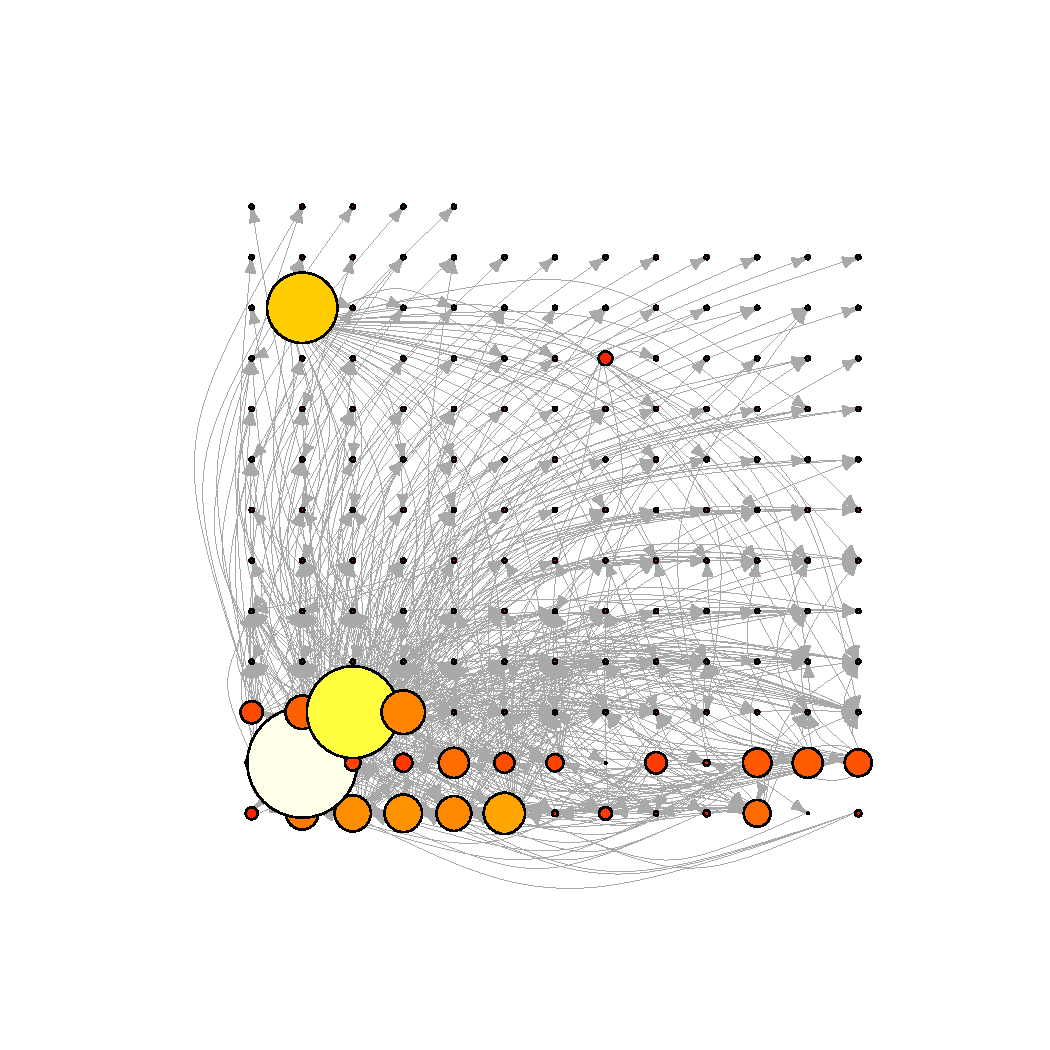
\includegraphics[trim = 30mm 30mm 30mm 30mm, clip, width=0.7\textwidth]{Images/Graph_Serengeti_Baskerville_tp.pdf}
\caption{The Serengeti food (\textit{Baskerville et al.}). Node sizes show out-degree / in-degree ratio;  node colours show node degree (as heat map).}
\end{figure}

Of the species studied by Baskerville et al. 129 are plants, 23 herbivores and 9 carnivores. Most of the links, 507, are between herbivores species and plants, while 85 are between animal species. The connectance of the graph is equal to $0.023$ is relatively small, compared to other food webs, and that was explained by the authors as a consequence of the higher taxonomic resolution of the plants species. The diameter of the food web as a directed graph is $2$ (is $6$ as a undirected graph).

Baskerville et al. computed a stochastic block partition of the food web, in a Bayesian framework where data and parameters are uncertain, where groups could have low or high within-connectance and between-connectance. The consensus partition of the groups identified 14 groups: two of carnivores, four of herbivores and eight of plants.

\begin{figure}[!ht]\label{fig:S_B_svds}
\centering
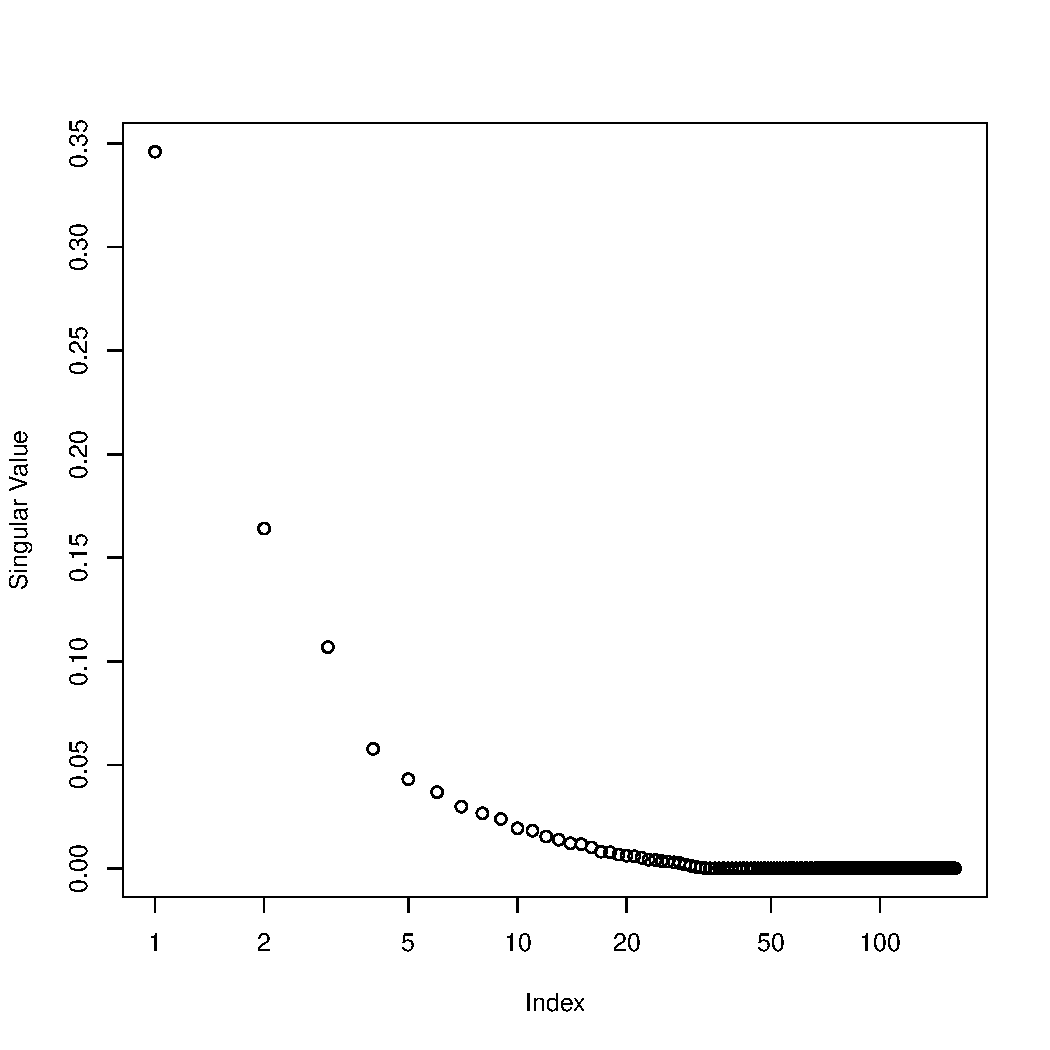
\includegraphics[width=0.5\textwidth]{Images/Svds_Serengeti_Baskerville.pdf}
\caption{Singular values of the adjacency matrix for the Baskerville's Serengeti food web.}
\end{figure}

From the sequence of the singular value of the Serengeti adjacency matrix, shown in figure~\ref{fig:S_B_svds}, we estimated that the optimal ranking dimension for the food web graph is between $d = 2$ and $d=4$

\todo[inline, color=green!40]{An ecologist may rise concerns how we choose the right ranking dimension.

My two cents: the choice can be based on the comparison between the SVD sequence of the food web analysed and a suitable neutral model random network. Here a \emph{suitable neutral model} is not a food wev theoretical model but a network where each node plays exactly the same role, has the same centrality and so on -- e.g., a toroidal lattice, an Erd\"{o}s-Renyi model, \dots. We consider those singular values that has a greater gap than what expected by the neutral model.

Do you think it may be a sensible approach?}

\begin{figure}[!htb]
\minipage{0.32\textwidth}
  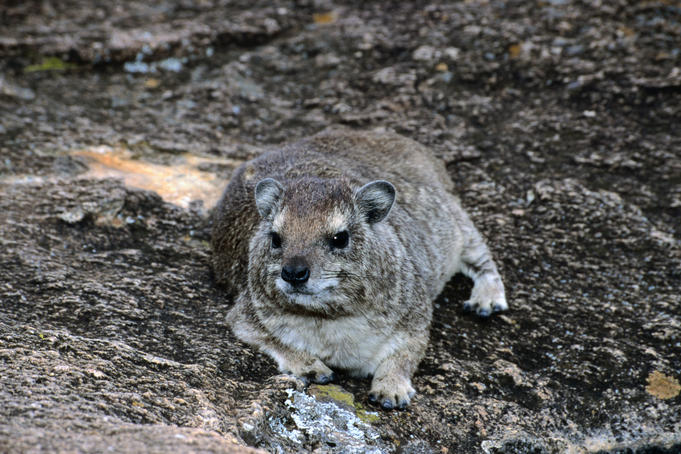
\includegraphics[width=\linewidth]{Images/Procavia.jpg}
\endminipage\hfill
\minipage{0.32\textwidth}
  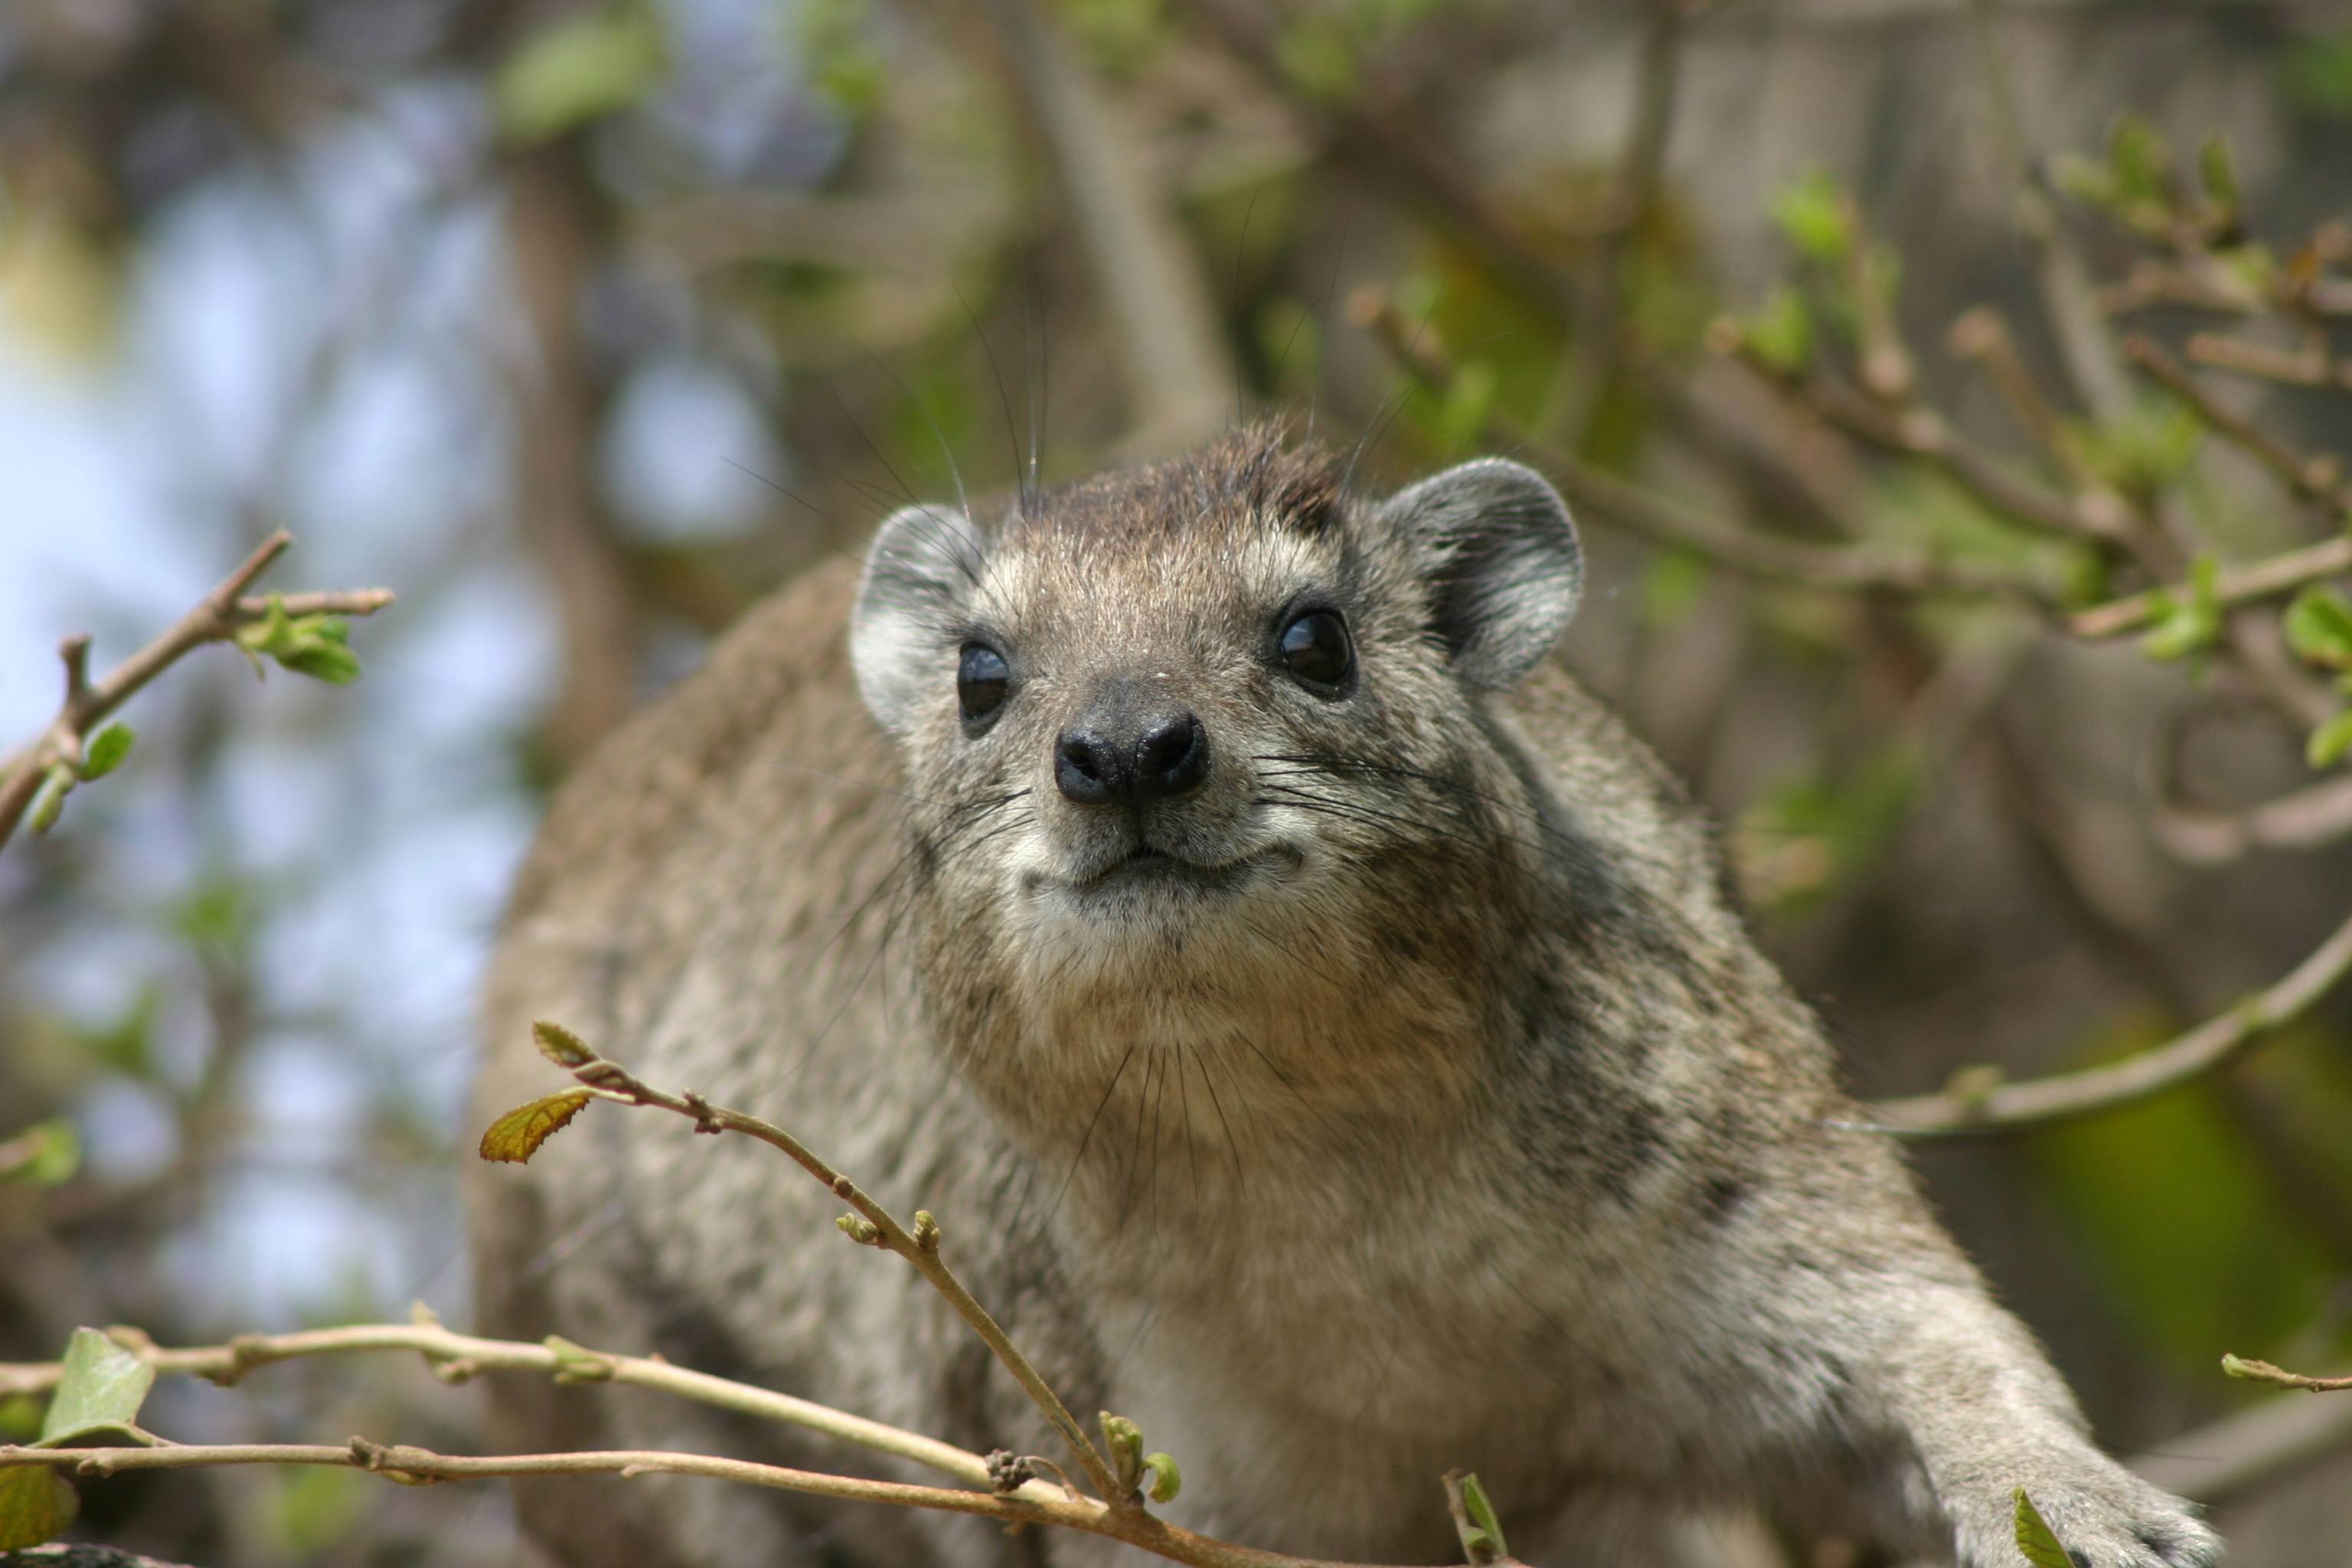
\includegraphics[width=\linewidth]{Images/Heterohyrax.jpg}
\endminipage\hfill
\minipage{0.32\textwidth}
  \includegraphics[width=\linewidth]{Images/Loxodonta_africana.jpg}
\endminipage
\caption{The three strongest embedding influence species (from the left \textit{Procavia Capensis}, \textit{Heterohyrax Brucei}, \textit{Loxodonta Africana}) in the Serengeti National Park based on the Baskerville et al. food web.}
\end{figure}

In ranking dimension $2$, the embedding influence has mean equal to $0.02677$, median equal to $0.00164$ and variance equal to $0.01665$. The $3$~stronger influenceing species are Procavia Capensis (the rock hyrax which embedding influence is equal to $1.3254$, that is around $50$ times the mean), Heterohyrax Brucei (the yellow-spotted rock hyrax which embedding influence is equal to $0.88876$) and Loxodonta Africana (the African bush elephant which embedding influence is equal to $0.31937$). The two hyrax constitute one of the 14 groups computed by \cite{baskerville2011spatial}, namely the group $5$. The African elephant is in the group $6$ with other 4 species. Both the hyrax are classified as {\em least concern} by the IUCN, while the African elephant is considered vulnerable, although its population its increasing.

The rank 2 embedding influence of the species in the Serengeti food web is shown in figure~\ref{fig:SSB2}.

\begin{figure}[!ht]\label{fig:SSB2}
\centering
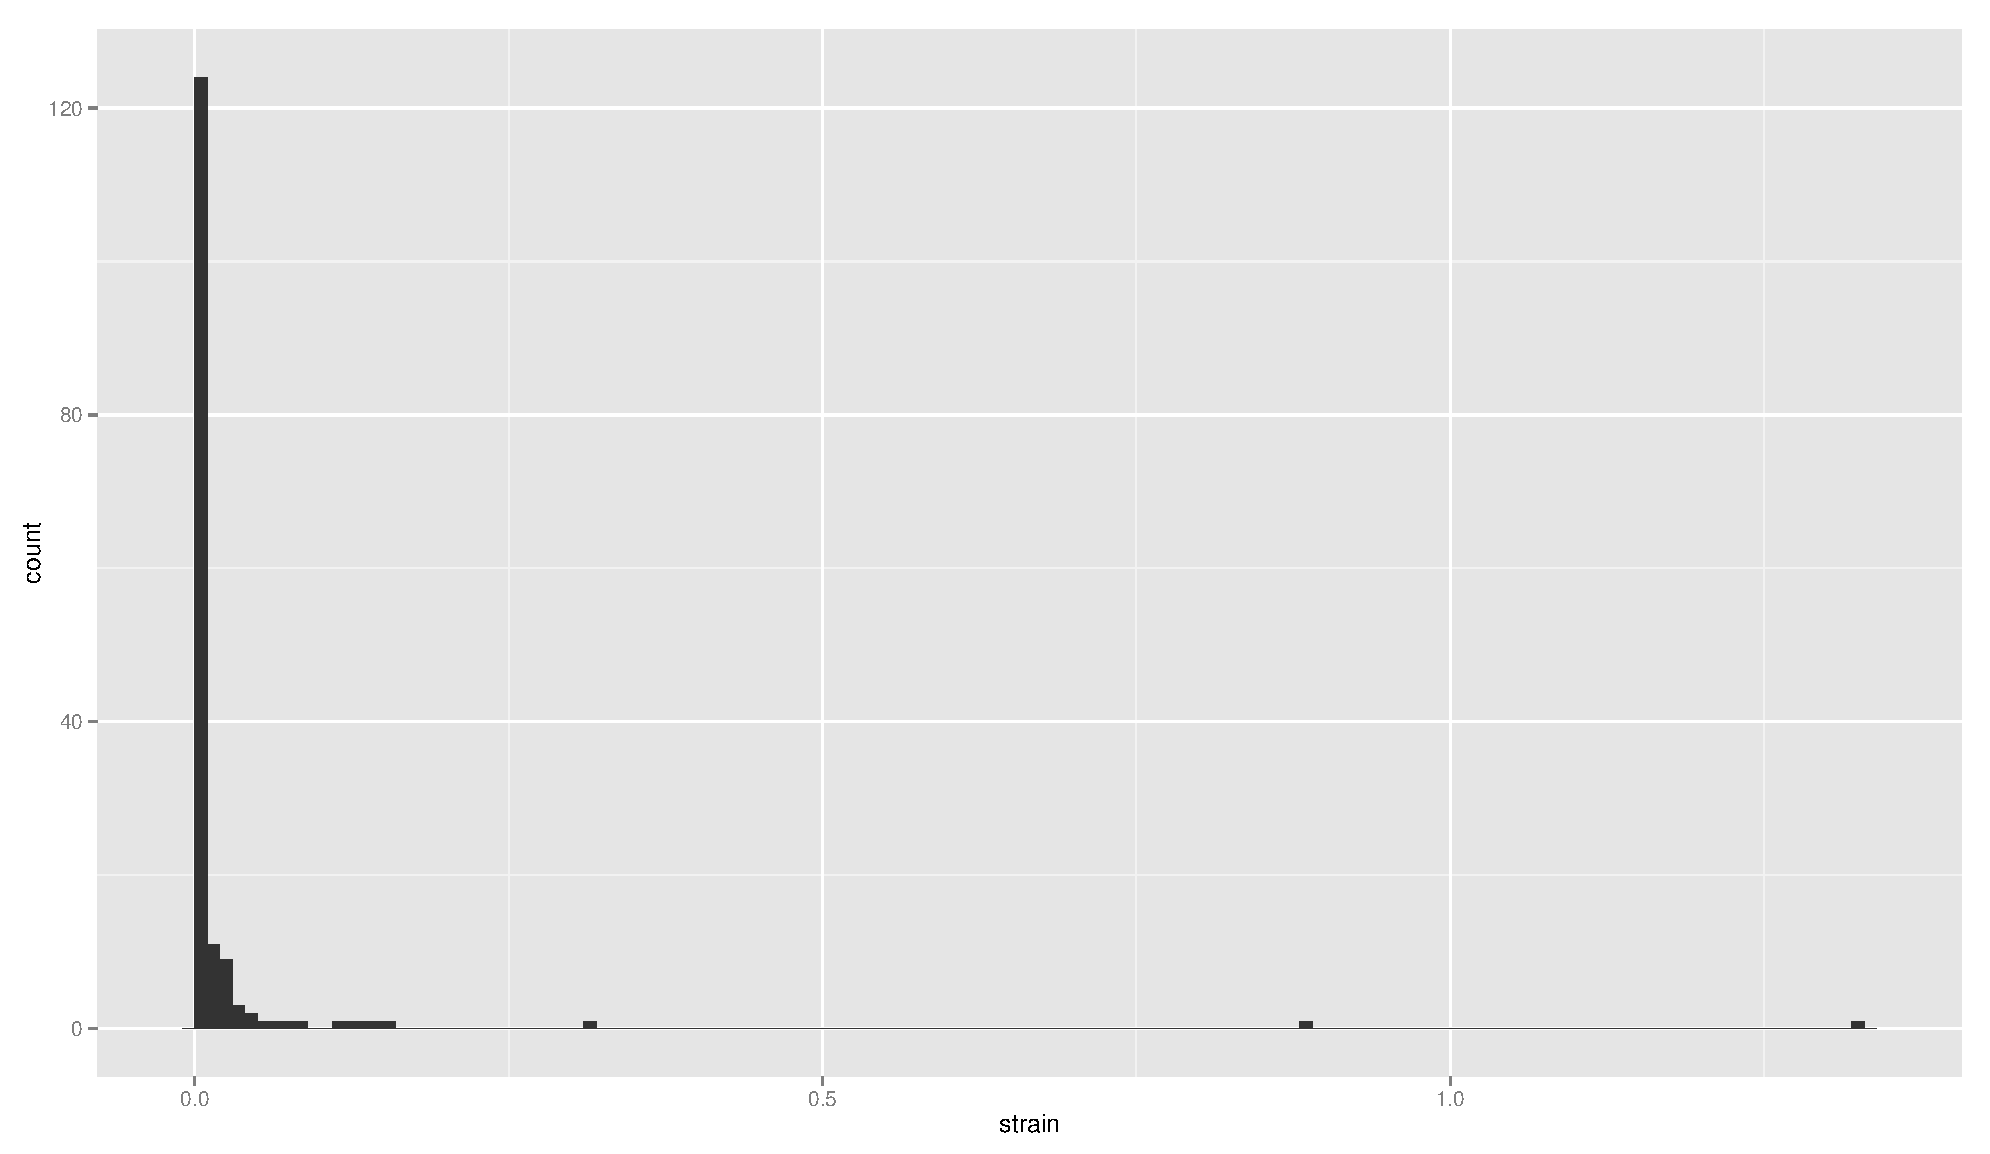
\includegraphics[height=0.3\textheight]{Images/influence_Serengeti_Baskerville_2.pdf}
\caption{Rank~$2$ embedding influence for the Serengeti food web.}
\end{figure}

Choosing a different embedding dimension we found consistency in the stronger influenceing species. For $d = 3$ the 3 stronger influenceing species were the same as for $d = 2$, while for $d = 4$ the 4 stronger influenceing species were (with decreasing influence) Loxodonta Africana, Procavia Capensis, Giraffa Camelopardalis (the giraffe, also in group $6$ as the elephant) and Heterohyrax Brucei.

\paragraph{de Visser et al.}
The Serengeti food web compiled by \cite{de2011serengeti} is populated by 86 species and 547 predation relationship. The connectance of the graph is equal to $0.07396$, more than three time the connectance found in the Baskerville et al. compilation. It is worth to say that the two food web are complementary and the overlap is little. The diameter of the food web both as a directed and as an undirected graph is $4$.

\begin{figure}[!ht]\label{fig:S_D}
\centering
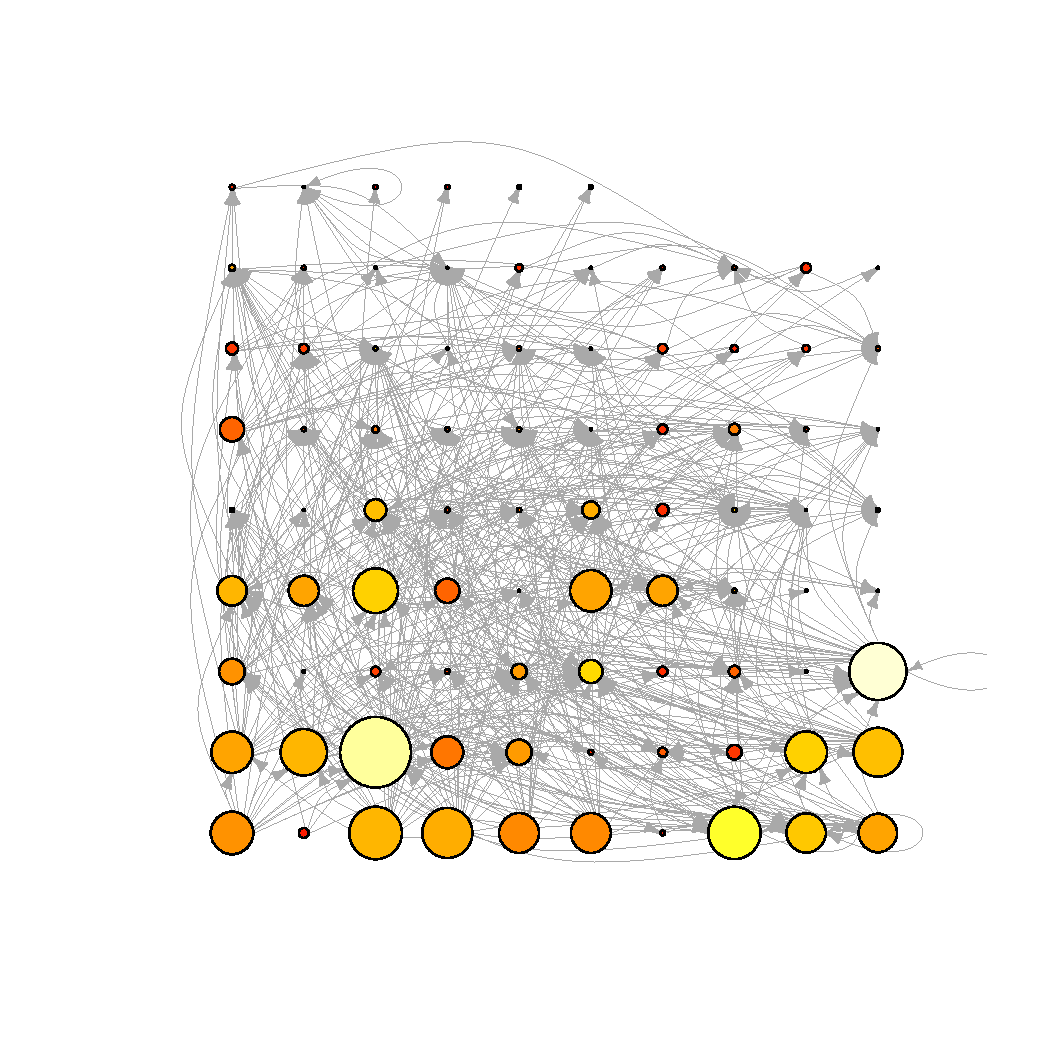
\includegraphics[trim = 30mm 25mm 20mm 25mm, clip, width=0.7\textwidth]{Images/Graph_Serengeti_deVisser.pdf}
\caption{The Serengeti food (\textit{de Visser et al.}). Node sizes show out-degree / in-degree ratio;  node colours show node degree (as heat map). }
\end{figure}

From the sequence of the singular value of the Serengeti adjacency matrix we estimated that the optimal ranking dimension for the food web graph is, again, between $d = 2$ and $d=4$. In ranking dimension $2$, the embedding influence takes values between $0.00009$ and $0.33118$, with mean equal to $0.05867$, median equal to $0.02959$ and variance equal to $0.00497$. The rank $2$ strongest influenceing species is the Heterohyrax Brucei. In the following position we find two nature resource, named by de Visser et al. ``Grass and herbs'' and ``Fruits and Nectar''. Again, we find consistent identification of the strongest influenceing species varying the embedding ranking, although it appears to be less strong than in the Baskerville et al. compilation.

The 10 stronger embedding influenceer for the Serengeti (\textit{de Visser et al.}) food web is given in table~\ref{tab:deVis}.

\begin{tabular}{c | c | c}\label{tab:deVis}
rank 2 & rank 3 & rank 4\\
Heterohyrax Brucei & Resource Grass & Heterohyrax Brucei\\
Resource Grains & Resource Crops & Dictyoptera\\
Resource Fruits & Resource Grains & Pelomys Fallax (creek rat)\\
Thripidae &  Resource Fruits & Resource Grains\\
Micropteropus pusillus & Heterohyrax Brucei & Steatomys pratensis\\
Diptera & Micropteropus pusillus & Apalis Flavida\\
Heteroptera & Hodotermes sp. & Resource Fruits\\
Lycaon pictus & Heteroptera & Resource Crops\\
Hodotermes sp. & Diptera & Orb-weaver Spiders\\
Madoqua kirkii & Helogale Parvula & Resource Grass
\end{tabular}

\todo[inline]{I removed the part on the Caribbean marine foodweb as it does not add any insight. Ready to ask if reviewers requires more examples.}
 

\subsection{Node network indexes and embedding influence}

In order to compare the embedding influence of a node with other known measures, we computed for each food web and each of the species present in the food web degree, out-degree, betweenness, closeness centrality, page rank and eigenvector centrality. Figure~\ref{fig:Scatter_S_B_2} shows a scatter plot of some of these measure against rank 2 embedding influence for the Serengeti (\textit{Baskerville et al.}) food web.\todo{There is an everyday longer and longer list for \emph{centralities} measures: ready to add or remove any particular one if requested.}

\begin{figure}[!ht]
\centering
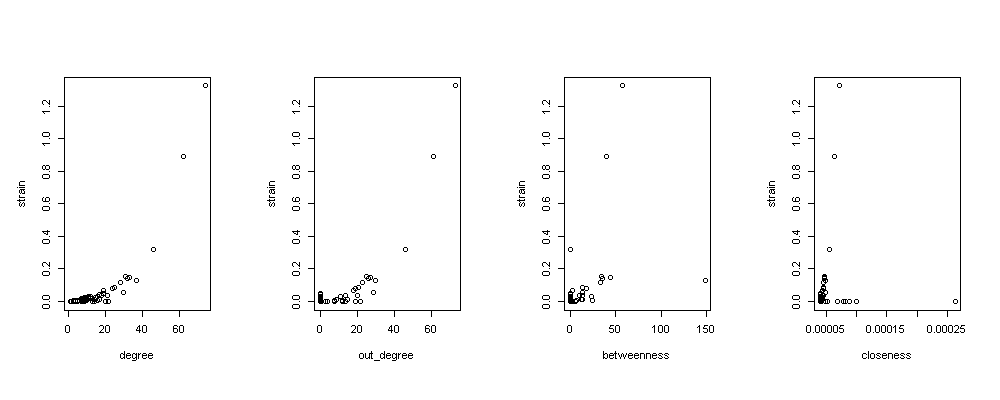
\includegraphics[width=\textwidth]{Images/Scatter_S_B_2.png}
\caption{Rank 2 embedding influence against (from the left) degree, out-degree, betweenness and closeness for the Serengeti (\textit{Baskerville et al.}) food web.}\label{fig:Scatter_S_B_2}
\end{figure}

We fitted these measures with the embedding influence for ranking dimension 2, 3 and 4. Figure~\ref{fig:rs_S_B_2} show the best linear regression models, for different model dimensions, for rank dimension 2, along with the coefficient of determination $R^2$, for the Serengeti Baskerville food web. In the appendix similar result are shown for the other food webs.
\begin{figure}[!htb]
\centering
  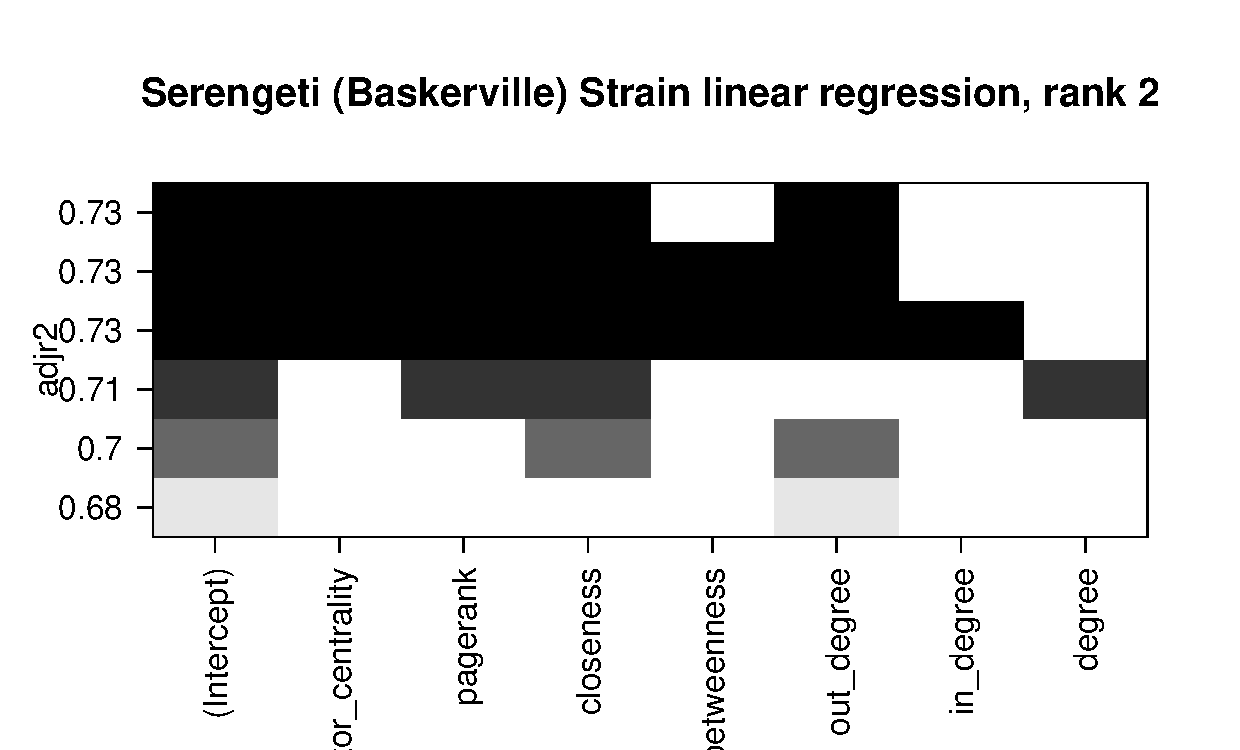
\includegraphics[width=\linewidth]{Images/B_S_R_2}
\caption{The best linear models for the Serengeti (\textit{Baskerville et al.} food web embedding influence, computed on the proposed measures for rank dimension 2.}\label{fig:rs_S_B_2}
\end{figure}

We didn't found any consistent signal across the various food webs analysed. Hence we argue that, although none of the previously stated measure is a good substitute, some measures, i.e., the out degree, the degree and the closeness centrality, play a role in defining the embedding influence of a node.

\section{Discussion}

\subsection{Motivations}
The motivation to consider a species reduced food web graph $G_{-i}$ and explore the embedding influence sequence $\underline{s(i)}$ arises in at least two real world case.

On the one hand the extinction of the species $v_i$: in this scenario we are interested in knowing how much the ecosystem has to adapt in order to support the species loss. On the other hand we know that the compilation of food webs is subject to errors and, hence, we can be interested in knowing how much a different picture we would have drawn if one of the species we know is there were not recorded.

\subsection{Further analysis}

\paragraph{Random generated graph embedding influence}
Although the degree of a node, and in second order its closeness centrality, appears as the best predictor within the proposed set of measures, the relationship between the more studied measures and the embedding influence remain to be explored and clarified. None of the existing measure appears to be equivalent to the embedding influence.

We already observed, in the empirical case proposed, the behaviour of the embedding influence compared to other network node statistics, often used to estimate the relative importance of a node in the graph.

In order to explore further a possible relationship, we computed the embedding influence sequence on different families of random network models, namely Erd\"{o}s-Renyi, Watts-Strogatz's Small-World and a random dot product mode with random vectors. We generated random network with a size and connectance comparable to that of the food webs previous introduced.

As for the empirical observed food webs, we fitted the previously stated node relative importance measures to the embedding influence.

\begin{small}
\bibliographystyle{plain}
\bibliography{asgefw}
\end{small}

\newpage

\appendix

\section{Stochastic blockmodels graph}

We introduced the embedding influence for random dot product food webs, but it's possible to give a definition of it in the more general framework of stochastic blockmodels graphs in a very similar way, assigning to every species in the same block the same latent vector.

The {\em stochastic blockmodel graph} is defined by the number of blocks $K$, the {\em block probability vector} $\rho \in \left(0,1\right]^K$ and the {\em communication probability matrix} $X \in \left[0,1\right]^{K \times K}$. The parameter $\rho$ satisfies $\sum_{k=1}^K\rho_k = 1$ while $X$ is \emph{identifiable}, that is for each $i,j \leq K$, $i \neq j$, the $i\mbox{th}$~row and the $j\mbox{th}$~row of $X$ are different and the $i\mbox{th}$~column and the $j\mbox{th}$~column of $X$ are different.

Each of the $n$ species is grouped in one of the blocks labelled $1, 2, \dots , K$. Thus, it's defined a {\em block membership function} $ \beta : V(G) \to \left\{ 1, 2, \dots , K \right\} $. The probability for a species $v_i$ to be grouped in block $k$ is given by $\rho_k$. Conditioned on the block membership function $\beta$, the probability that there exist an edge $\left( v_i, v_j \right)$ is given by $X_{\beta{(v_i)},\beta{(v_j)}}$ and is independent from the other couples of species. The model can be generalised to the case where there are $S$ probability community matrices.

Consider the adjacency matrix $A_G$ observed for the foodweb $G$ as a particular outcome of a stochastic blockmodel graph adjacency matrix of which we don't know the parameters nor the block membership function.

The rank~$d$ singular value decomposition of the matrix $A_G \in \{0,1\}^{n^2}$ is the given of the six matrices
\[
\{U,U_d,S,S_d,V,V_d\}
\]
with $U, V \in \RR^{n \times d}$, $U_d,V_d \in \RR^{n \times (n-d})$, $S \in \RR^{d \times d}$, $S_d \in \RR^{(n-d)\times (n-d)}$, such that
\[
A_G = \left[ U | U_d \right] \left( S \oplus S_d \right) \left[ V | V_d \right]
\]
where $\left[ U | U_d \right]$, which columns are called the left-singular vectors of $A_G$, and  $\left[ V | V_d \right]$, which columns are called the right-singular vectors of $A_G$, are real orthogonal matrices, while $\Sigma = S \oplus S_d$ is the diagonal matrix of the singular values of $A_G$, i.e. a diagonal matrix with descending entries $\Sigma^{1,1} \geq \Sigma^{2,2} \geq \dots \geq \Sigma^{n,n}$.

Define $\sqrt{S} \in \RR^{d \times d}$ as the diagonal matrix with entries are the square roots of the diagonal entries of $S$. Then we define $L$ and $R$ as $U \sqrt{S}$ and $V \sqrt{S}$ respectively.

We can, now, cluster the rows of $L$ or $R$ or $\left[ L | R \right]$ into at most $d$ clusters under the minimum least squares criterion (but other algorithm could be used): if the rows of $X$ are pairwise different, compute
\[
\RR^{n \times d} \ni \hat{X} := \min_{M \in \RR^{n \times d}} || M - L ||_F
\]
where the matrices $M$ have at most $K$ distinct rows; if the columns of $X$ are pairwise different, compute
\[
\RR^{n \times d} \ni \hat{X} := \min_{M \in \RR^{n \times d}} || M - R ||_F
\]
where the matrices $M$ have at most $K$ distinct rows; otherwise compute
\[
\RR^{n \times 2d} \ni \hat{X} := \min_{M \in \RR^{n \times 2d}} || M - \left[ L | R \right]||_F
\]
where the matrices $M$ have at most $K$ distinct rows. The clusters so computed give a consistent estimates for the true graph blocks.

We are now able to define the embedding influence as the distance between $\hat{X}_{G - i}$ and $\hat{X}^{- i}$.

\newpage

\section{Food webs network analysis}

We computed degree, in-degree, out-degree, betweenness, closeness centrality, page rank and eigenvector centrality using R 3.0.3 \cite{team2012r} and the packages \emph{igraph}  \cite{Csardiigraph}, \emph{shapes}, \emph{ppls}, \emph{ggplot2}, \emph{car}, \emph{leaps} (\textbf{REFS!!!}).

\begin{figure}[ht]\label{fig:Serengeti_embeddingstress_d2}
\centering
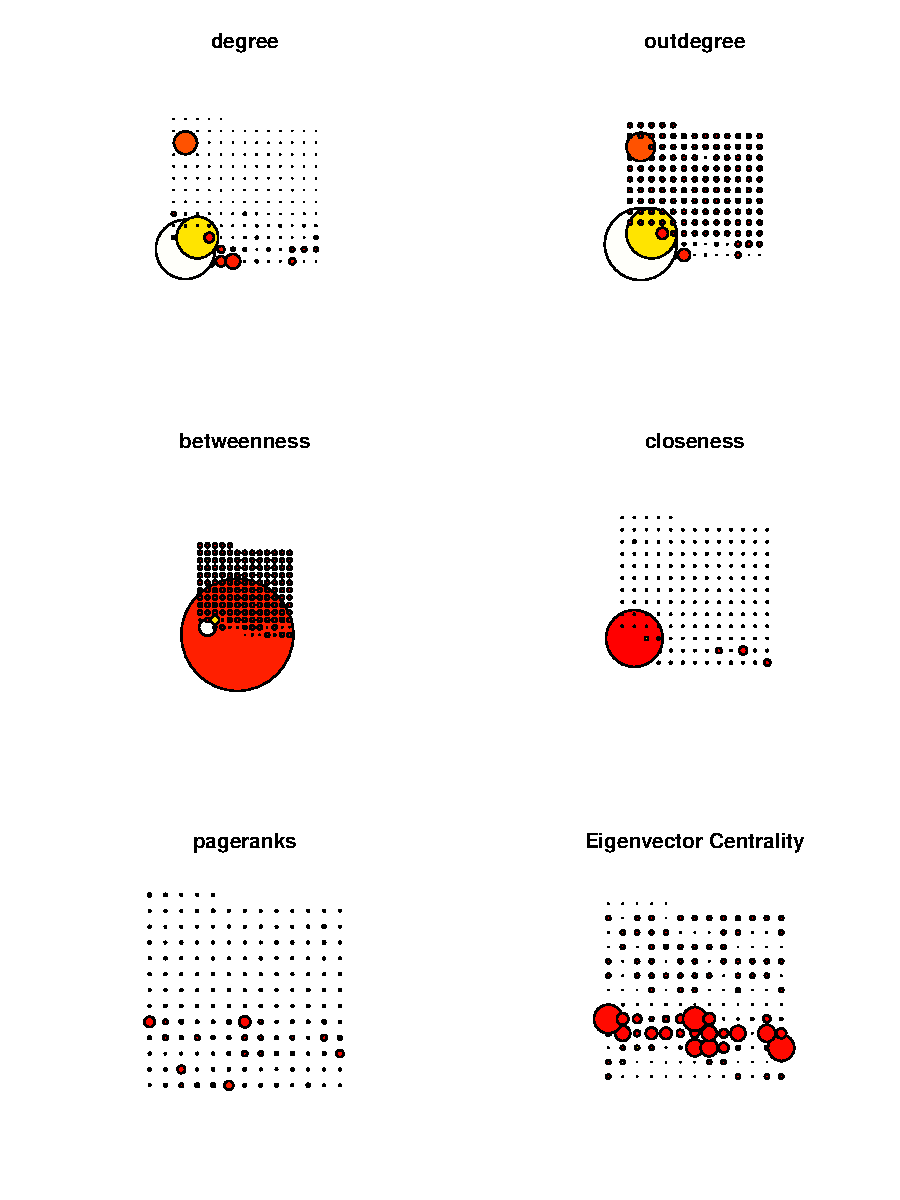
\includegraphics[width=0.7\textwidth]{Images/influence_statistics_Serengeti_Baskerville_2.pdf}
\caption{This plots offer a graphic representation of the rank~$2$ embedding influence of nodes, as a colour in the heat map, compared to other nodes measures, as size, for the Serengeti (Baskerville et al.) food web.}
\end{figure}


\end{document}